\documentclass[]{article}
\usepackage{lmodern}
\usepackage{amssymb,amsmath}
\usepackage{ifxetex,ifluatex}
\usepackage{fixltx2e} % provides \textsubscript
\ifnum 0\ifxetex 1\fi\ifluatex 1\fi=0 % if pdftex
  \usepackage[T1]{fontenc}
  \usepackage[utf8]{inputenc}
\else % if luatex or xelatex
  \ifxetex
    \usepackage{mathspec}
  \else
    \usepackage{fontspec}
  \fi
  \defaultfontfeatures{Ligatures=TeX,Scale=MatchLowercase}
\fi
% use upquote if available, for straight quotes in verbatim environments
\IfFileExists{upquote.sty}{\usepackage{upquote}}{}
% use microtype if available
\IfFileExists{microtype.sty}{%
\usepackage{microtype}
\UseMicrotypeSet[protrusion]{basicmath} % disable protrusion for tt fonts
}{}
\usepackage[margin=1in]{geometry}
\usepackage{hyperref}
\hypersetup{unicode=true,
            pdftitle={Chapter 2 - Summarizing Data},
            pdfborder={0 0 0},
            breaklinks=true}
\urlstyle{same}  % don't use monospace font for urls
\usepackage{graphicx,grffile}
\makeatletter
\def\maxwidth{\ifdim\Gin@nat@width>\linewidth\linewidth\else\Gin@nat@width\fi}
\def\maxheight{\ifdim\Gin@nat@height>\textheight\textheight\else\Gin@nat@height\fi}
\makeatother
% Scale images if necessary, so that they will not overflow the page
% margins by default, and it is still possible to overwrite the defaults
% using explicit options in \includegraphics[width, height, ...]{}
\setkeys{Gin}{width=\maxwidth,height=\maxheight,keepaspectratio}
\IfFileExists{parskip.sty}{%
\usepackage{parskip}
}{% else
\setlength{\parindent}{0pt}
\setlength{\parskip}{6pt plus 2pt minus 1pt}
}
\setlength{\emergencystretch}{3em}  % prevent overfull lines
\providecommand{\tightlist}{%
  \setlength{\itemsep}{0pt}\setlength{\parskip}{0pt}}
\setcounter{secnumdepth}{0}
% Redefines (sub)paragraphs to behave more like sections
\ifx\paragraph\undefined\else
\let\oldparagraph\paragraph
\renewcommand{\paragraph}[1]{\oldparagraph{#1}\mbox{}}
\fi
\ifx\subparagraph\undefined\else
\let\oldsubparagraph\subparagraph
\renewcommand{\subparagraph}[1]{\oldsubparagraph{#1}\mbox{}}
\fi

%%% Use protect on footnotes to avoid problems with footnotes in titles
\let\rmarkdownfootnote\footnote%
\def\footnote{\protect\rmarkdownfootnote}

%%% Change title format to be more compact
\usepackage{titling}

% Create subtitle command for use in maketitle
\providecommand{\subtitle}[1]{
  \posttitle{
    \begin{center}\large#1\end{center}
    }
}

\setlength{\droptitle}{-2em}

  \title{Chapter 2 - Summarizing Data}
    \pretitle{\vspace{\droptitle}\centering\huge}
  \posttitle{\par}
    \author{}
    \preauthor{}\postauthor{}
    \date{}
    \predate{}\postdate{}
  
\usepackage{geometry}
\usepackage{multicol}
\usepackage{multirow}

\begin{document}
\maketitle

\textbf{Stats scores}. (2.33, p.~78) Below are the final exam scores of
twenty introductory statistics students.

57, 66, 69, 71, 72, 73, 74, 77, 78, 78, 79, 79, 81, 81, 82, 83, 83, 88,
89, 94

Create a box plot of the distribution of these scores. The five number
summary provided below may be useful.

\begin{center}
\renewcommand\arraystretch{1.5}
\begin{tabular}{ccccc}
Min & Q1    & Q2 (Median)   & Q3    & Max \\
\hline
57  & 72.5  & 78.5          & 82.5  & 94 \\
\end{tabular}
\end{center}

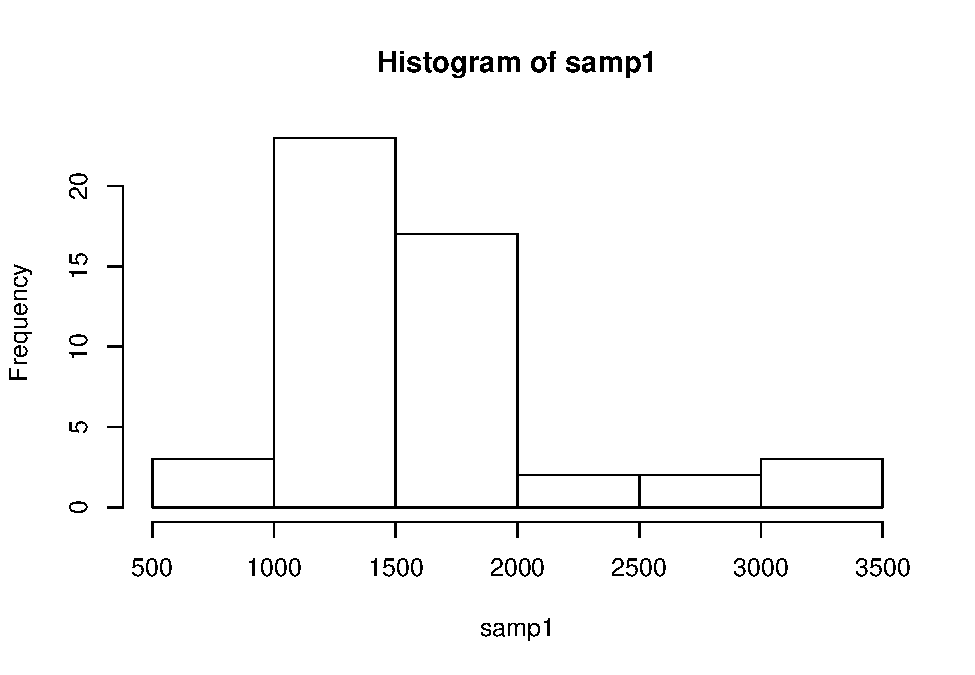
\includegraphics{Homework2_files/figure-latex/unnamed-chunk-1-1.pdf}

\begin{center}\rule{0.5\linewidth}{\linethickness}\end{center}

\clearpage

\textbf{Mix-and-match}. (2.10, p.~57) Describe the distribution in the
histograms below and match them to the box plots.

\includegraphics{Homework2_files/figure-latex/unnamed-chunk-2-1.pdf}

\begin{center}\rule{0.5\linewidth}{\linethickness}\end{center}

\clearpage

\textbf{Distributions and appropriate statistics, Part II}. (2.16,
p.~59) For each of the following, state whether you expect the
distribution to be symmetric, right skewed, or left skewed. Also specify
whether the mean or median would best represent a typical observation in
the data, and whether the variability of observations would be best
represented using the standard deviation or IQR. Explain your reasoning.

\begin{enumerate}
\def\labelenumi{(\alph{enumi})}
\tightlist
\item
  Housing prices in a country where 25\% of the houses cost below
  \$350,000, 50\% of the houses cost below \$450,000, 75\% of the houses
  cost below \$1,000,000 and there are a meaningful number of houses
  that cost more than \$6,000,000.
\item
  Housing prices in a country where 25\% of the houses cost below
  \$300,000, 50\% of the houses cost below \$600,000, 75\% of the houses
  cost below \$900,000 and very few houses that cost more than
  \$1,200,000.
\item
  Number of alcoholic drinks consumed by college students in a given
  week. Assume that most of these students don’t drink since they are
  under 21 years old, and only a few drink excessively.
\item
  Annual salaries of the employees at a Fortune 500 company where only a
  few high level executives earn much higher salaries than the all other
  employees.
\end{enumerate}

\begin{center}\rule{0.5\linewidth}{\linethickness}\end{center}

\clearpage

\textbf{Heart transplants.} (2.26, p.~76) The Stanford University Heart
Transplant Study was conducted to determine whether an experimental
heart transplant program increased lifespan. Each patient entering the
program was designated an official heart transplant candidate, meaning
that he was gravely ill and would most likely benefit from a new heart.
Some patients got a transplant and some did not. The variable
\emph{transplant} indicates which group the patients were in; patients
in the treatment group got a transplant and those in the control group
did not. Of the 34 patients in the control group, 30 died. Of the 69
people in the treatment group, 45 died. Another variable called
\emph{survived} was used to indicate whether or not the patient was
alive at the end of the study.

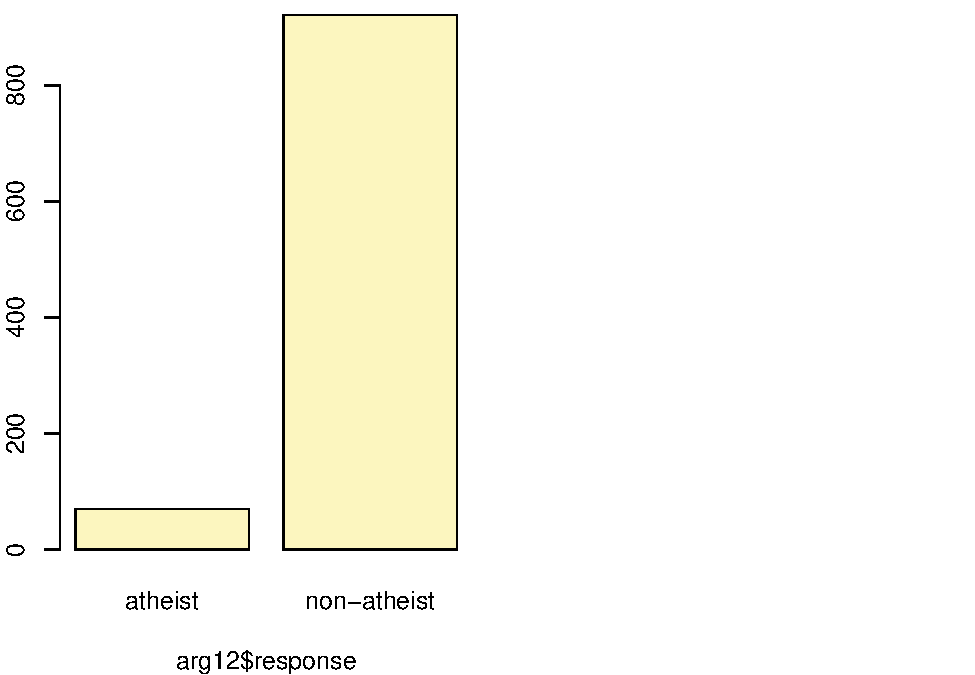
\includegraphics[width=0.5\linewidth]{Homework2_files/figure-latex/unnamed-chunk-3-1}
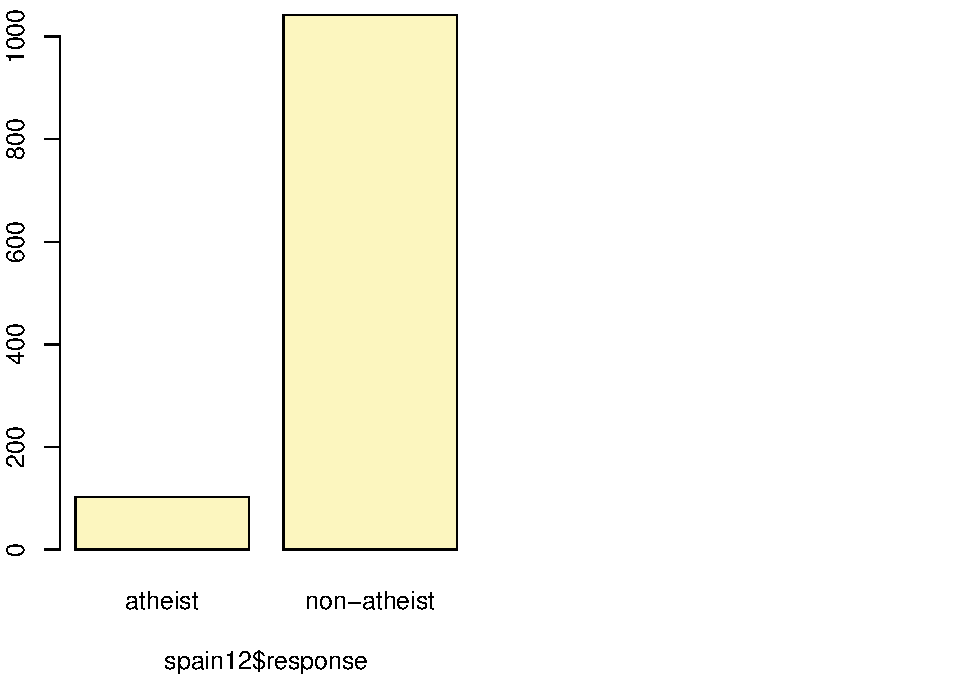
\includegraphics[width=0.5\linewidth]{Homework2_files/figure-latex/unnamed-chunk-3-2}

\begin{enumerate}
\def\labelenumi{(\alph{enumi})}
\tightlist
\item
  Based on the mosaic plot, is survival independent of whether or not
  the patient got a transplant? Explain your reasoning.
\item
  What do the box plots below suggest about the efficacy (effectiveness)
  of the heart transplant treatment.
\item
  What proportion of patients in the treatment group and what proportion
  of patients in the control group died?
\item
  One approach for investigating whether or not the treatment is
  effective is to use a randomization technique.
\end{enumerate}

\begin{enumerate}
\def\labelenumi{\roman{enumi}.}
\tightlist
\item
  What are the claims being tested?
\item
  The paragraph below describes the set up for such approach, if we were
  to do it without using statistical software. Fill in the blanks with a
  number or phrase, whichever is appropriate.
\end{enumerate}

\begin{quote}
We write \emph{alive} on \_\_\_\_\_\_\_\_\_\_ cards representing
patients who were alive at the end of the study, and \emph{dead} on
\_\_\_\_\_\_\_\_\_ cards representing patients who were not. Then, we
shuffle these cards and split them into two groups: one group of size
\_\_\_\_\_\_\_\_\_ representing treatment, and another group of size
\_\_\_\_\_\_\_\_\_\_ representing control. We calculate the difference
between the proportion of \emph{dead} cards in the treatment and control
groups (treatment - control) and record this value. We repeat this 100
times to build a distribution centered at \_\_\_\_\_\_\_\_\_. Lastly, we
calculate the fraction of simulations where the simulated differences in
proportions are \_\_\_\_\_\_\_\_\_. If this fraction is low, we conclude
that it is unlikely to have observed such an outcome by chance and that
the null hypothesis should be rejected in favor of the alternative.
\end{quote}

\begin{enumerate}
\def\labelenumi{\roman{enumi}.}
\setcounter{enumi}{2}
\tightlist
\item
  What do the simulation results shown below suggest about the
  effectiveness of the transplant program?
\end{enumerate}

\begin{center}

\includegraphics[width=0.75\linewidth]{Homework2_files/figure-latex/unnamed-chunk-5-1} 
\end{center}


\end{document}
